% Figure 4.10  (label fig:cfghub_map)
% Caption: \texttt{cfg\_hub} 64\,KB Address Map.
% Extracted standalone source of the TikZ figure embedded in MARS_碩士論文.tex
% Compile: pdflatex fig4.10_cfghub_map.tex
\documentclass[border=6pt]{standalone}
\usepackage{tikz}
\usetikzlibrary{shapes.geometric, arrows.meta, positioning, fit, backgrounds, calc, decorations.pathreplacing}
\begin{document}
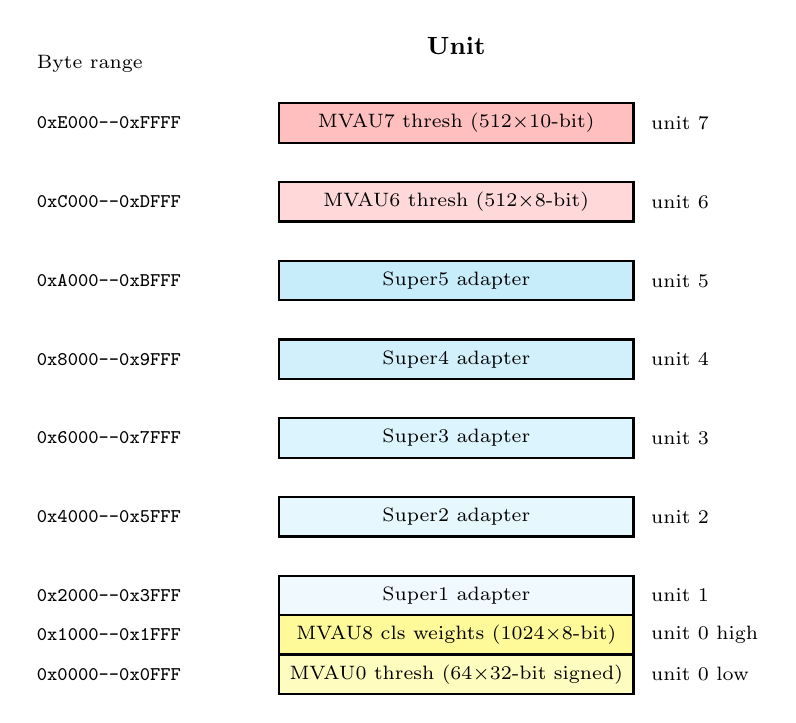
\begin{tikzpicture}[font=\footnotesize]
\foreach \y/\range/\label/\col in {%
    7/0xE000--0xFFFF/MVAU7 thresh (512$\times$10-bit)/red!25,
    6/0xC000--0xDFFF/MVAU6 thresh (512$\times$8-bit)/red!15,
    5/0xA000--0xBFFF/Super5 adapter/cyan!22,
    4/0x8000--0x9FFF/Super4 adapter/cyan!18,
    3/0x6000--0x7FFF/Super3 adapter/cyan!14,
    2/0x4000--0x5FFF/Super2 adapter/cyan!10,
    1/0x2000--0x3FFF/Super1 adapter/cyan!6,
    0.5/0x1000--0x1FFF/MVAU8 cls weights (1024$\times$8-bit)/yellow!40,
    0/0x0000--0x0FFF/MVAU0 thresh (64$\times$32-bit signed)/yellow!25
} {
    \draw[fill=\col, thick] (0,\y) rectangle (4.5,\y+0.5);
    \node[anchor=west, font=\scriptsize\ttfamily] at (-3.2,\y+0.25) {\range};
    \node[font=\scriptsize] at (2.25,\y+0.25) {\label};
}
\node[font=\small\bfseries, anchor=south] at (2.25, 8) {Unit};
\node[anchor=west, font=\scriptsize] at (-3.2, 8) {Byte range};
\foreach \y/\u in {0/0 low, 0.5/0 high, 1/1, 2/2, 3/3, 4/4, 5/5, 6/6, 7/7} {
    \node[anchor=west, font=\scriptsize] at (4.6,\y+0.25) {unit \u};
}
\end{tikzpicture}
\end{document}
